% DO NOT COMPILE THIS FILE DIRECTLY!
% This is included by the other .tex files.

\begin{frame}[t,plain]
\titlepage
\end{frame}

\begin{frame}[t]{Bayesian Inference How-To}
As the title suggests, this session will be {\bf practical}.
\vspace{1cm}

We will study a selection of techniques that you can use to solve any
inference problem that comes your way!
\end{frame}

\begin{frame}[t]{That said...}
It is inevitable that I will state some opinions and philosophies!\\
{\bf We can't help it.}
\end{frame}

\begin{frame}[t]{Python}
Examples will be given in Python, and will use {\tt numpy} for numerical
things (arrays, random number generation), and {\tt matplotlib} for plotting.\\
\vspace{1cm}
Code should work in either Python 2 or 3.
\end{frame}

\begin{frame}[t, fragile]{Python}
All code will assume the following {\tt import} statements.
\begin{minted}[mathescape,
               numbersep=5pt,
               gobble=2,
               frame=lines,
               framesep=2mm]{python}
  import numpy as np
  import numpy.random as rng
  import matplotlib.pyplot as plt
  import copy
\end{minted}
\end{frame}


\begin{frame}[t, fragile]{Python}
When I code in Python, I have a C++ accent. Here's a habit that might
seem strange:

\begin{minted}[mathescape,
               numbersep=5pt,
               gobble=2,
               frame=lines,
               framesep=2mm]{python}
  x = 4  # I know this is an integer
  y = 5. # This is a float because of the decimal point.
\end{minted}
\end{frame}


\begin{frame}[t]{Emphasis}
I will try to emphasise the underlying ideas of the methods.\\
I will not
be teaching specific software packages
(e.g. {\it emcee}, {\it MultiNest}, {\it DNest3}), though I may mention them.
\end{frame}

\begin{frame}[t]{Ingredients I}
Bayesian inference need the following inputs:

\begin{itemize}
\setlength{\itemsep}{20pt}
\item A {\bf hypothesis space} describing the set of possible answers to our
question (``parameter space'' in fitting is the same concept).
\item A {\bf prior distribution} $p(\theta)$ describing how plausible
each of the possible solutions is, not taking into account the data.
\end{itemize}
\end{frame}

\begin{frame}[t]{Ingredients II}
Bayesian inference need the following inputs:
\begin{itemize}
\item A {\bf sampling distribution} $p(D | \theta)$ describing our knowledge
about the connection between the parameters and the data.
\end{itemize}

When $D$ is known,
this is a function of $\theta$ called the {\bf likelihood}.
\end{frame}


\begin{frame}[t]{The Posterior Distribution}
The data helps us by changing our prior distribution to the {\bf posterior
distribution}, given by
\begin{eqnarray}
p(\theta | D) &=& \frac{p(\theta) p(D|\theta)}{p(D)}
\end{eqnarray}
where the denominator is the normalisation constant, usually called either
the {\bf marginal likelihood} or the {\bf evidence}.
\begin{eqnarray}
p(D) &=& \int p(\theta)p(D|\theta) \, d\theta.
\end{eqnarray}

\end{frame}


\begin{frame}[t]{The Logic of the Updating Process}
A standard ``medical testing'' example, when a diagnostic test is only
95\% accurate (i.e. there is a 5\% probability it indicates you have
the disease when you don't, and vice versa).

$H$ = You have the disease\\
$D$ = You test positive for the disease

\end{frame}




\begin{frame}[t]{Parameter Estimation}
What is a parameter?

\begin{itemize}
\item A quantity whose value you would like to know; or
\item A quantity you think you need in order to write down
$p(D | \theta)$.
\end{itemize}

The latter are often called {\bf nuisance parameters}.
\end{frame}

\begin{frame}[t]{Transit Example}
\begin{figure}
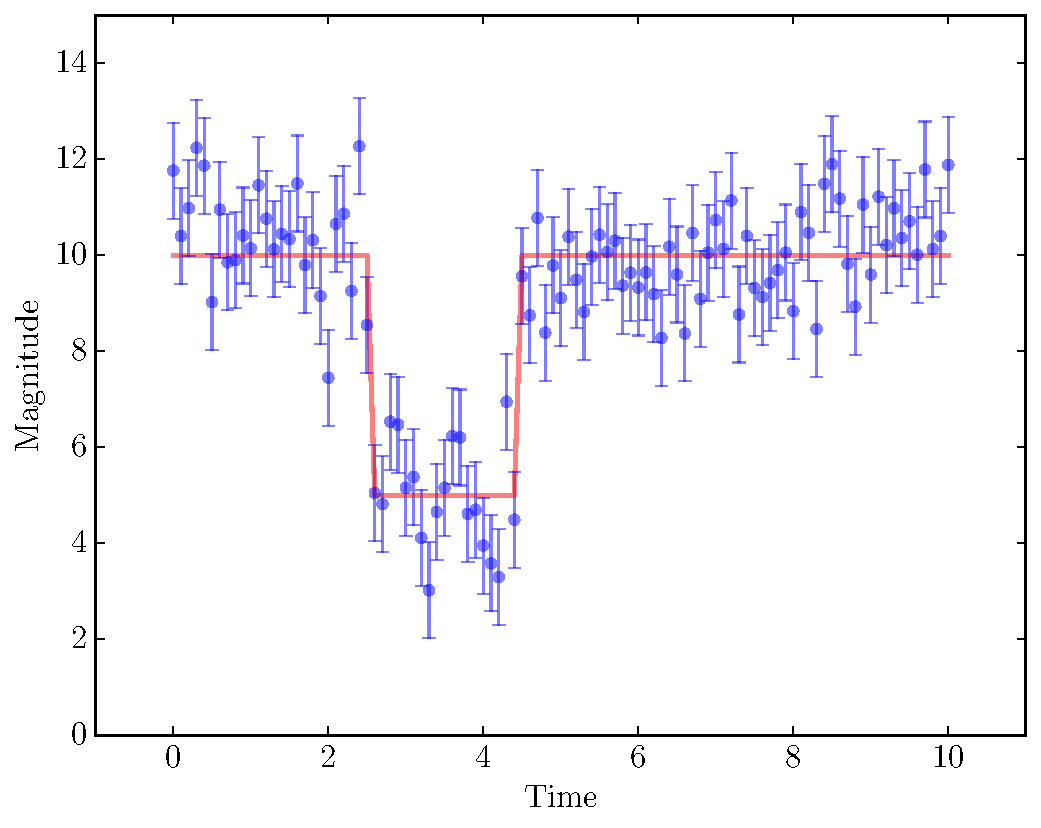
\includegraphics[scale=0.4]{Code/transit_data.pdf}
\end{figure}
\end{frame}

\begin{frame}[t]{Transit Example: The Truth}
The red curve was:
\begin{eqnarray}
\mu(t) &=& \left\{
\begin{array}{lr}
10, & 2.5 \leq t \leq 4.5\\
5,  & \textnormal{otherwise}.
\end{array}
\right.
\end{eqnarray}

\begin{figure}
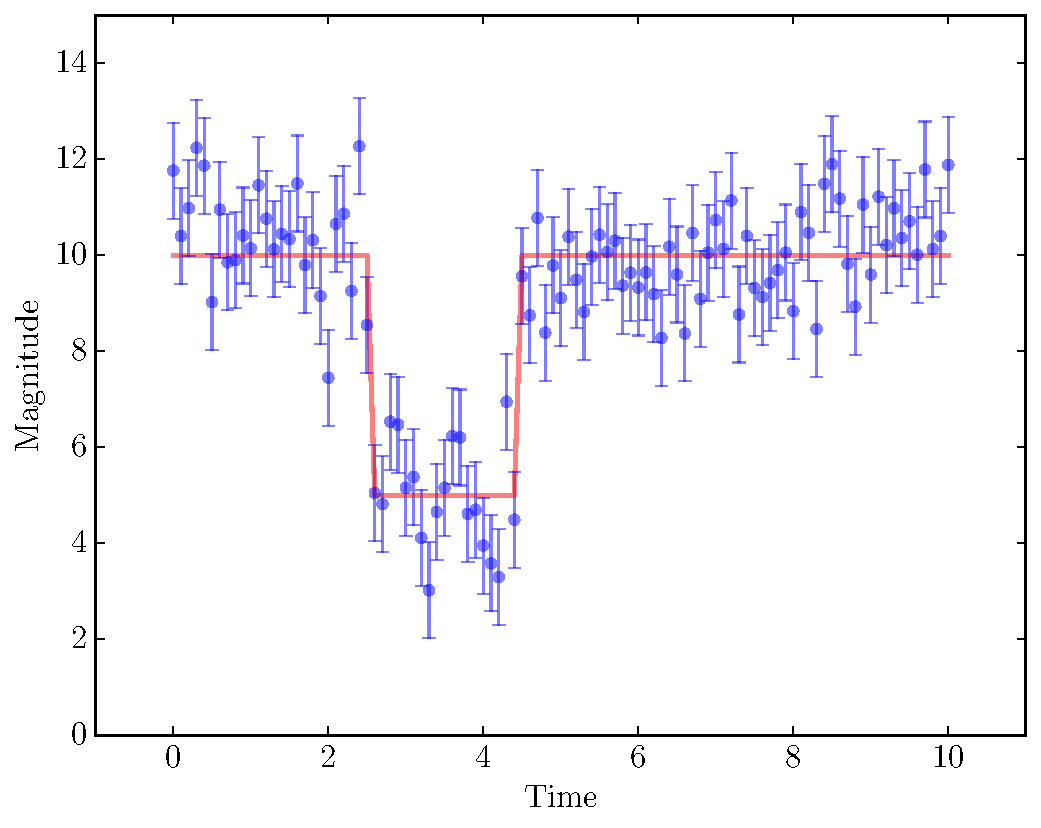
\includegraphics[scale=0.3]{Code/transit_data.pdf}
\end{figure}
\end{frame}

\begin{frame}[fragile, t]{Transit Example: The Truth}
The red curve was:
\begin{eqnarray}
\mu(t) &=& \left\{
\begin{array}{lr}
10, & 2.5 \leq t \leq 4.5\\
5,  & \textnormal{otherwise}.
\end{array}
\right.
\end{eqnarray}

and the noise was generated like this:
\begin{minted}[mathescape,
               numbersep=5pt,
               gobble=2,
               frame=lines,
               framesep=2mm]{python}
  # Add noise
  sig = 1.
  y += sig*rng.randn(y.size)
\end{minted}
\end{frame}



\begin{frame}[t]{Transit Example}
This example is quite simple, yet it is complex enough to demonstrate many
important principles.
\vspace{1cm}

It is also closely related to many astronomical situations!
\end{frame}


\begin{frame}[t]{Related to the transit example...}
\begin{itemize}
\item Realistic exoplanet transits
\item Finding emission/absorption lines in spectra
\item Finding stars/galaxies in an image
\item ¡Y mucho más!
\end{itemize}
\end{frame}

